\section{Design}\label{sec: Design}
In this section the design and decisions that where made to achieve the laboratory are discussed.

\subsection{ATM machine Part I}\label{subsec: ATM machine Part I}
The software of the previous lab has been split up into two files so that the main logic and main program flow is in the main file and the functions are separated in an atm\_func file. Furthermore a file I/O for login errors was implemented to aid assistance by unusual behavior. The two code listening are shown in Listening \ref{lst: Python code for an ATM Part I} nad \ref{lst: Python functions for an ATM Part I}. A single function is shown in Listening \ref{lst: Python function mainMenu}.

\begin{lstlisting}[style=PythonStyle, language=Python, caption={Python function mainMenu .},label=lst: Python function mainMenu ]
def mainMenue ( ) :
	print ( " Main Menu" )
	print ( "------------------------ \n" )
	print ( " 1 . CHECK BALANCE" )
	print ( " 2 . WITHDRAW CASH" )
	print ( " 3 . DEPOSIT CASH" )
	print ( " 4 . CHANGE PIN" )
	print ( " 5 . EXIT " )
	return 1 # no error 1 , error 0
\end{lstlisting}

The following Listening shows the function call in the main program. That shows how bigger programs in python can be structured sequentially.

\begin{lstlisting}[style=PythonStyle, language=Python, caption={Python function call mainMenu .},label=lst: Python function call mainMenu ]
mainMenue () 
\end{lstlisting}
The following listening shows the error log output file content. This can be easily used to check which errors has been tested and has a message generated to it. The error log is continuously appended into a text file and has to be managed manually so far this can be automated with a script as example.
\begin{lstlisting}[ caption={Error log Part II.},label=lst: Error log Part II ]
Thu Oct 25 09:15:45 2018ATM program starts 
Thu Oct 25 09:15:54 2018 User logged in 
Thu Oct 25 09:16:06 2018 Withdraw error
Thu Oct 25 09:16:19 2018 Deposit error
Thu Oct 25 09:16:34 2018 User PIN error
Thu Oct 25 09:27:05 2018 Program Closed
\end{lstlisting}

\subsection{ATM machine Part II}\label{subsec: ATM machine Part II}
In this part the program was expended with an receipt function that would log all the transactions of a ongoing section and let the user decide to print it out the end of the session. Figure \ref{fig: Printed receipt} shows how the user can decide after exiting the program if he wishes to print the receipt or not. The python code himself for file I/O used can be examen in closer detail in Listening \ref{lst: Python code for an ATM Part II} and \ref{lst: Python code for an ATM Part II functions}. First a file has to be open this can be done with open(<filename>, mode) and then be accessed with the functions .read() and .write(). 

\begin{figure}[H]
	\centering
	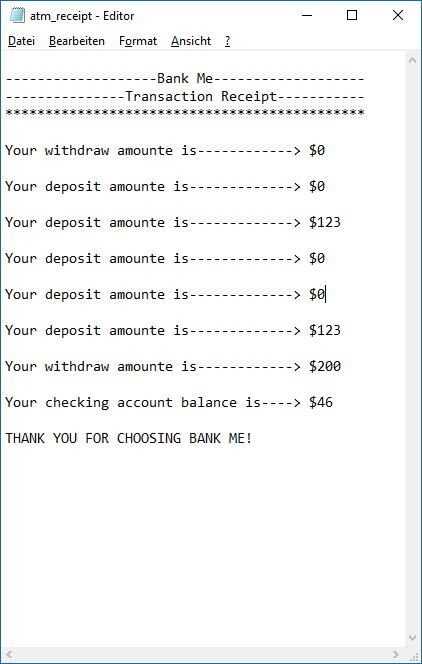
\includegraphics[width=0.5\textwidth]{01_images/printed_receipt.PNG}
	\caption{Printed receipt.}
	\label{fig: Printed receipt}
\end{figure}
Listening \ref{lst: Python file I/O example} shows how a text file can be opened either with append mode or write mode. It shows also how errors can be handled with try and except commands. The lowest line show how to close a file.
\begin{lstlisting}[style=PythonStyle, language=Python, caption={Python file I/O example.},label=lst: Python file I/O example ]
# Open a file
try:
	fo = open("07_lab_error_log.txt", "a")
	fr = open(atm.ReceiptFile, "w")
	fo.write(asctime()+ ' ATM program starts '+ '\n')
	fr.write('\n-------------------Bank Me-------------------\n')
	fr.write('---------------Transaction Receipt-----------\n')
	fr.write('*********************************************\n\n')
except IOError as e:
	print('File '+e.filename+' could not be opened or writen to!') 

fo.write(asctime()+ ' Program Closed\n')
fo.close() # to ensure file is closed
fr.close() # to ensure file is closed
\end{lstlisting}

\subsection{ATM machine Part III}\label{subsec: ATM machine Part III}
This section shall demonstrated the objective programming that allows two crate a class an instance this class as instances or an instance. A class contains usually data objects and methods. Listening \ref{lst: Python class example with a method} shows the class named Atm with class variables followed by the \_\_init\_\_ function which is first call after instantiation of a class and serves to initializes specific variables. next the normal statements or so called methods are listed which can be used in the main program. Notice, the word $self$ which is used in a method which defines a method and separate it from a normal static function.

\begin{lstlisting}[style=PythonStyle, language=Python, caption={Python class example with a method.},label=lst: Python class example with a method ]
import re
class Atm:
	AMOUNT_MIN = 0
	AMOUNT_MAX = 1000
	
	Pin  = "1234"
	Select = 0
	AccountValue = 0
	ReceiptFile = "atm_receipt.txt"
	
	def __init__(self, AccountValue, Pin):
		self.AccountValue = AccountValue
		self.Pin = Pin
	
	# Print Receipt
	def receipt(self, filename, file):
		file.write('THANK YOU FOR CHOOSING BANK ME!')
		file.close()
		file = open(filename, "r")
		for line in file:
		print(line, end='')
		file.close()
		return 1
\end{lstlisting}
Listening \ref{lst: Python object example with a method} shows how a class can be imported with from import command and how it can be instantiated with initial variables as an object called atm. It also shows how methods can be used as example atm.welcome(). Class variables can be accessed like atm.Pin as example.
\begin{lstlisting}[style=PythonStyle, language=Python, caption={Python object example with a method.},label=lst: Python object example with a method ]
from atm_class import Atm
atm = Atm(100,'2345') # instantiate class Atm to atm object

# Star program
if atm.welcome(): # first method used from the atm object
	error = 0 
else:
	error = 1
	fo.write(asctime()+ ' welcome() error\n')

# PIN validation
while True:
	ret = 0
	if atm.pin( input("Please enter your PIN: "), atm.Pin): 
		error = 0 
		fo.write(asctime()+ ' User logged in \n')
		break   
	else:
		error = 1
		fo.write(asctime()+ ' User login error\n')
\end{lstlisting}
The following listening shows the error log output file content. This can be easily used to check which errors has been tested and has a message generated to it. The error log is continuously appended into a text file and has to be managed manually so far this can be automated with a script as example. 
\begin{lstlisting}[ caption={Error log Part III.},label=lst: Error log Part III ]
Thu Oct 25 15:53:33 2018 ATM program starts 
Thu Oct 25 15:53:37 2018 User login error
Thu Oct 25 15:53:40 2018 User login error
Thu Oct 25 15:53:44 2018 User login error
Thu Oct 25 15:53:46 2018 User login error
Thu Oct 25 15:53:48 2018 User logged in 
Thu Oct 25 15:54:13 2018 Deposit error
Thu Oct 25 15:54:26 2018 Deposit error
Thu Oct 25 15:54:54 2018 Withdraw error
Thu Oct 25 15:55:00 2018 Withdraw error
Thu Oct 25 15:56:47 2018 Program Closed
\end{lstlisting}
Figure \ref{fig: printed_receipt_partIII} shows the receipt output generated by the program written in part three where a class of an ATM was instantiated instead of functions methods where used.This together with the error log confirms the correct functioning of the ATM.
\begin{figure}[H]
	\centering
	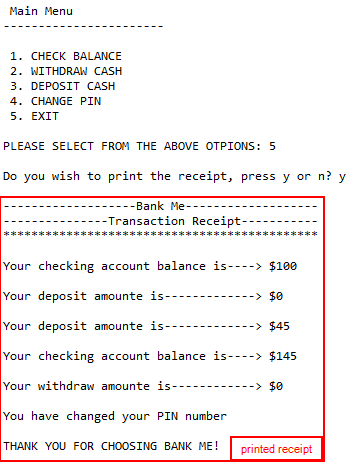
\includegraphics[width=0.5\textwidth]{01_images/printed_receipt_partIII.PNG}
	\caption{Printed receipt Part III.}
	\label{fig: printed_receipt_partIII}
\end{figure}

Further work would be to write the file I/O access in better methods which makes it nicer to look and easier to handle as well as the error log handling is still plumb and needs a better strategy if the program would be advanced.